\documentclass[twoside]{book}

% Packages required by doxygen
\usepackage{fixltx2e}
\usepackage{calc}
\usepackage{doxygen}
\usepackage[export]{adjustbox} % also loads graphicx
\usepackage{graphicx}
\usepackage[utf8]{inputenc}
\usepackage{makeidx}
\usepackage{multicol}
\usepackage{multirow}
\PassOptionsToPackage{warn}{textcomp}
\usepackage{textcomp}
\usepackage[nointegrals]{wasysym}
\usepackage[table]{xcolor}

% Font selection
\usepackage[T1]{fontenc}
\usepackage[scaled=.90]{helvet}
\usepackage{courier}
\usepackage{amssymb}
\usepackage{sectsty}
\renewcommand{\familydefault}{\sfdefault}
\allsectionsfont{%
  \fontseries{bc}\selectfont%
  \color{darkgray}%
}
\renewcommand{\DoxyLabelFont}{%
  \fontseries{bc}\selectfont%
  \color{darkgray}%
}
\newcommand{\+}{\discretionary{\mbox{\scriptsize$\hookleftarrow$}}{}{}}

% Page & text layout
\usepackage{geometry}
\geometry{%
  a4paper,%
  top=2.5cm,%
  bottom=2.5cm,%
  left=2.5cm,%
  right=2.5cm%
}
\tolerance=750
\hfuzz=15pt
\hbadness=750
\setlength{\emergencystretch}{15pt}
\setlength{\parindent}{0cm}
\setlength{\parskip}{3ex plus 2ex minus 2ex}
\makeatletter
\renewcommand{\paragraph}{%
  \@startsection{paragraph}{4}{0ex}{-1.0ex}{1.0ex}{%
    \normalfont\normalsize\bfseries\SS@parafont%
  }%
}
\renewcommand{\subparagraph}{%
  \@startsection{subparagraph}{5}{0ex}{-1.0ex}{1.0ex}{%
    \normalfont\normalsize\bfseries\SS@subparafont%
  }%
}
\makeatother

% Headers & footers
\usepackage{fancyhdr}
\pagestyle{fancyplain}
\fancyhead[LE]{\fancyplain{}{\bfseries\thepage}}
\fancyhead[CE]{\fancyplain{}{}}
\fancyhead[RE]{\fancyplain{}{\bfseries\leftmark}}
\fancyhead[LO]{\fancyplain{}{\bfseries\rightmark}}
\fancyhead[CO]{\fancyplain{}{}}
\fancyhead[RO]{\fancyplain{}{\bfseries\thepage}}
\fancyfoot[LE]{\fancyplain{}{}}
\fancyfoot[CE]{\fancyplain{}{}}
\fancyfoot[RE]{\fancyplain{}{\bfseries\scriptsize Generated by Doxygen }}
\fancyfoot[LO]{\fancyplain{}{\bfseries\scriptsize Generated by Doxygen }}
\fancyfoot[CO]{\fancyplain{}{}}
\fancyfoot[RO]{\fancyplain{}{}}
\renewcommand{\footrulewidth}{0.4pt}
\renewcommand{\chaptermark}[1]{%
  \markboth{#1}{}%
}
\renewcommand{\sectionmark}[1]{%
  \markright{\thesection\ #1}%
}

% Indices & bibliography
\usepackage{natbib}
\usepackage[titles]{tocloft}
\setcounter{tocdepth}{3}
\setcounter{secnumdepth}{5}
\makeindex

% Hyperlinks (required, but should be loaded last)
\usepackage{ifpdf}
\ifpdf
  \usepackage[pdftex,pagebackref=true]{hyperref}
\else
  \usepackage[ps2pdf,pagebackref=true]{hyperref}
\fi
\hypersetup{%
  colorlinks=true,%
  linkcolor=blue,%
  citecolor=blue,%
  unicode%
}

% Custom commands
\newcommand{\clearemptydoublepage}{%
  \newpage{\pagestyle{empty}\cleardoublepage}%
}

\usepackage{caption}
\captionsetup{labelsep=space,justification=centering,font={bf},singlelinecheck=off,skip=4pt,position=top}

%===== C O N T E N T S =====

\begin{document}

% Titlepage & ToC
\hypersetup{pageanchor=false,
             bookmarksnumbered=true,
             pdfencoding=unicode
            }
\pagenumbering{alph}
\begin{titlepage}
\vspace*{7cm}
\begin{center}%
{\Large Implicit and Explicit Scheme \\[1ex]\large 1.\+0.\+0 }\\
\vspace*{1cm}
{\large Generated by Doxygen 1.8.14}\\
\end{center}
\end{titlepage}
\clearemptydoublepage
\pagenumbering{roman}
\tableofcontents
\clearemptydoublepage
\pagenumbering{arabic}
\hypersetup{pageanchor=true}

%--- Begin generated contents ---
\chapter{Hierarchical Index}
\section{Class Hierarchy}
This inheritance list is sorted roughly, but not completely, alphabetically\+:\begin{DoxyCompactList}
\item \contentsline{section}{Scheme}{\pageref{class_scheme}}{}
\begin{DoxyCompactList}
\item \contentsline{section}{Explicit\+Scheme}{\pageref{class_explicit_scheme}}{}
\item \contentsline{section}{Implicit\+Scheme}{\pageref{class_implicit_scheme}}{}
\end{DoxyCompactList}
\item vector\begin{DoxyCompactList}
\item \contentsline{section}{Matrix}{\pageref{class_matrix}}{}
\end{DoxyCompactList}
\end{DoxyCompactList}

\chapter{Class Index}
\section{Class List}
Here are the classes, structs, unions and interfaces with brief descriptions\+:\begin{DoxyCompactList}
\item\contentsline{section}{\mbox{\hyperlink{class_explicit_scheme}{Explicit\+Scheme}} }{\pageref{class_explicit_scheme}}{}
\item\contentsline{section}{\mbox{\hyperlink{class_implicit_scheme}{Implicit\+Scheme}} }{\pageref{class_implicit_scheme}}{}
\item\contentsline{section}{\mbox{\hyperlink{class_matrix}{Matrix}} }{\pageref{class_matrix}}{}
\item\contentsline{section}{\mbox{\hyperlink{class_scheme}{Scheme}} }{\pageref{class_scheme}}{}
\end{DoxyCompactList}

\chapter{Class Documentation}
\hypertarget{class_explicit_scheme}{}\section{Explicit\+Scheme Class Reference}
\label{class_explicit_scheme}\index{Explicit\+Scheme@{Explicit\+Scheme}}


{\ttfamily \#include $<$Explicit\+Scheme.\+h$>$}



Inheritance diagram for Explicit\+Scheme\+:
% FIG 0


Collaboration diagram for Explicit\+Scheme\+:
% FIG 1
\subsection*{Public Member Functions}
\begin{DoxyCompactItemize}
\item 
\mbox{\hyperlink{class_explicit_scheme_ae63cfb8d333897b625dd17dc2acb4c46}{Explicit\+Scheme}} ()
\item 
string \mbox{\hyperlink{class_explicit_scheme_a52c0d19315a6014f43a9d007c70582d6}{Explicit\+Up\+Wind\+F\+T\+BS}} ()
\item 
string \mbox{\hyperlink{class_explicit_scheme_a2698e08e62763c56b972b478d665c34c}{Explicit\+Lax\+Wandroff}} ()
\item 
\mbox{\hyperlink{class_explicit_scheme_a5eee023f6f9d09609066a50dd620b49a}{$\sim$\+Explicit\+Scheme}} ()
\end{DoxyCompactItemize}
\subsection*{Additional Inherited Members}


\subsection{Detailed Description}
Inherited class, which includes implicit schemes like Up Wind Forward-\/\+Time Backward-\/\+Space and Forward-\/\+Time Central-\/\+Space. Additionally, class includes private method with Thomas Algorithm. 

\subsection{Constructor \& Destructor Documentation}
\mbox{\Hypertarget{class_explicit_scheme_ae63cfb8d333897b625dd17dc2acb4c46}\label{class_explicit_scheme_ae63cfb8d333897b625dd17dc2acb4c46}} 
\index{Explicit\+Scheme@{Explicit\+Scheme}!Explicit\+Scheme@{Explicit\+Scheme}}
\index{Explicit\+Scheme@{Explicit\+Scheme}!Explicit\+Scheme@{Explicit\+Scheme}}
\subsubsection{\texorpdfstring{Explicit\+Scheme()}{ExplicitScheme()}}
{\footnotesize\ttfamily Explicit\+Scheme\+::\+Explicit\+Scheme (\begin{DoxyParamCaption}{ }\end{DoxyParamCaption})}

Default, empty constructor for \mbox{\hyperlink{class_explicit_scheme}{Explicit\+Scheme}} class. \mbox{\Hypertarget{class_explicit_scheme_a5eee023f6f9d09609066a50dd620b49a}\label{class_explicit_scheme_a5eee023f6f9d09609066a50dd620b49a}} 
\index{Explicit\+Scheme@{Explicit\+Scheme}!````~Explicit\+Scheme@{$\sim$\+Explicit\+Scheme}}
\index{````~Explicit\+Scheme@{$\sim$\+Explicit\+Scheme}!Explicit\+Scheme@{Explicit\+Scheme}}
\subsubsection{\texorpdfstring{$\sim$\+Explicit\+Scheme()}{~ExplicitScheme()}}
{\footnotesize\ttfamily Explicit\+Scheme\+::$\sim$\+Explicit\+Scheme (\begin{DoxyParamCaption}{ }\end{DoxyParamCaption})}

Default, empty destructor for \mbox{\hyperlink{class_explicit_scheme}{Explicit\+Scheme}} class. Here is the caller graph for this function\+:
% FIG 2


\subsection{Member Function Documentation}
\mbox{\Hypertarget{class_explicit_scheme_a2698e08e62763c56b972b478d665c34c}\label{class_explicit_scheme_a2698e08e62763c56b972b478d665c34c}} 
\index{Explicit\+Scheme@{Explicit\+Scheme}!Explicit\+Lax\+Wandroff@{Explicit\+Lax\+Wandroff}}
\index{Explicit\+Lax\+Wandroff@{Explicit\+Lax\+Wandroff}!Explicit\+Scheme@{Explicit\+Scheme}}
\subsubsection{\texorpdfstring{Explicit\+Lax\+Wandroff()}{ExplicitLaxWandroff()}}
{\footnotesize\ttfamily string Explicit\+Scheme\+::\+Explicit\+Lax\+Wandroff (\begin{DoxyParamCaption}{ }\end{DoxyParamCaption})}

Public method, which solves the difference using explicit scheme Lax-\/\+Wandroff \begin{DoxyReturn}{Returns}
string -\/ name of method for saving result into files with proper name 
\end{DoxyReturn}
\begin{DoxySeeAlso}{See also}
\mbox{\hyperlink{class_scheme_ae4512b4c8ead4d8ced95174f0b241f8a}{Save\+Result\+Into\+Files(double delta\+T, string scheme\+Name)}} 
\end{DoxySeeAlso}
Here is the caller graph for this function\+:
% FIG 3
\mbox{\Hypertarget{class_explicit_scheme_a52c0d19315a6014f43a9d007c70582d6}\label{class_explicit_scheme_a52c0d19315a6014f43a9d007c70582d6}} 
\index{Explicit\+Scheme@{Explicit\+Scheme}!Explicit\+Up\+Wind\+F\+T\+BS@{Explicit\+Up\+Wind\+F\+T\+BS}}
\index{Explicit\+Up\+Wind\+F\+T\+BS@{Explicit\+Up\+Wind\+F\+T\+BS}!Explicit\+Scheme@{Explicit\+Scheme}}
\subsubsection{\texorpdfstring{Explicit\+Up\+Wind\+F\+T\+B\+S()}{ExplicitUpWindFTBS()}}
{\footnotesize\ttfamily string Explicit\+Scheme\+::\+Explicit\+Up\+Wind\+F\+T\+BS (\begin{DoxyParamCaption}{ }\end{DoxyParamCaption})}

Public method, which solves the difference using explicit scheme Up Wind Forward-\/\+Time Backward-\/\+Space \begin{DoxyReturn}{Returns}
string -\/ name of method for saving result into files with proper name 
\end{DoxyReturn}
\begin{DoxySeeAlso}{See also}
\mbox{\hyperlink{class_scheme_ae4512b4c8ead4d8ced95174f0b241f8a}{Save\+Result\+Into\+Files(double delta\+T, string scheme\+Name)}} 
\end{DoxySeeAlso}
Here is the caller graph for this function\+:
% FIG 4


The documentation for this class was generated from the following files\+:\begin{DoxyCompactItemize}
\item 
\mbox{\hyperlink{_explicit_scheme_8h}{Explicit\+Scheme.\+h}}\item 
\mbox{\hyperlink{_explicit_scheme_8cpp}{Explicit\+Scheme.\+cpp}}\end{DoxyCompactItemize}

\hypertarget{class_implicit_scheme}{}\section{Implicit\+Scheme Class Reference}
\label{class_implicit_scheme}\index{Implicit\+Scheme@{Implicit\+Scheme}}


{\ttfamily \#include $<$Implicit\+Scheme.\+h$>$}

Inheritance diagram for Implicit\+Scheme\+:\begin{figure}[H]
\begin{center}
\leavevmode
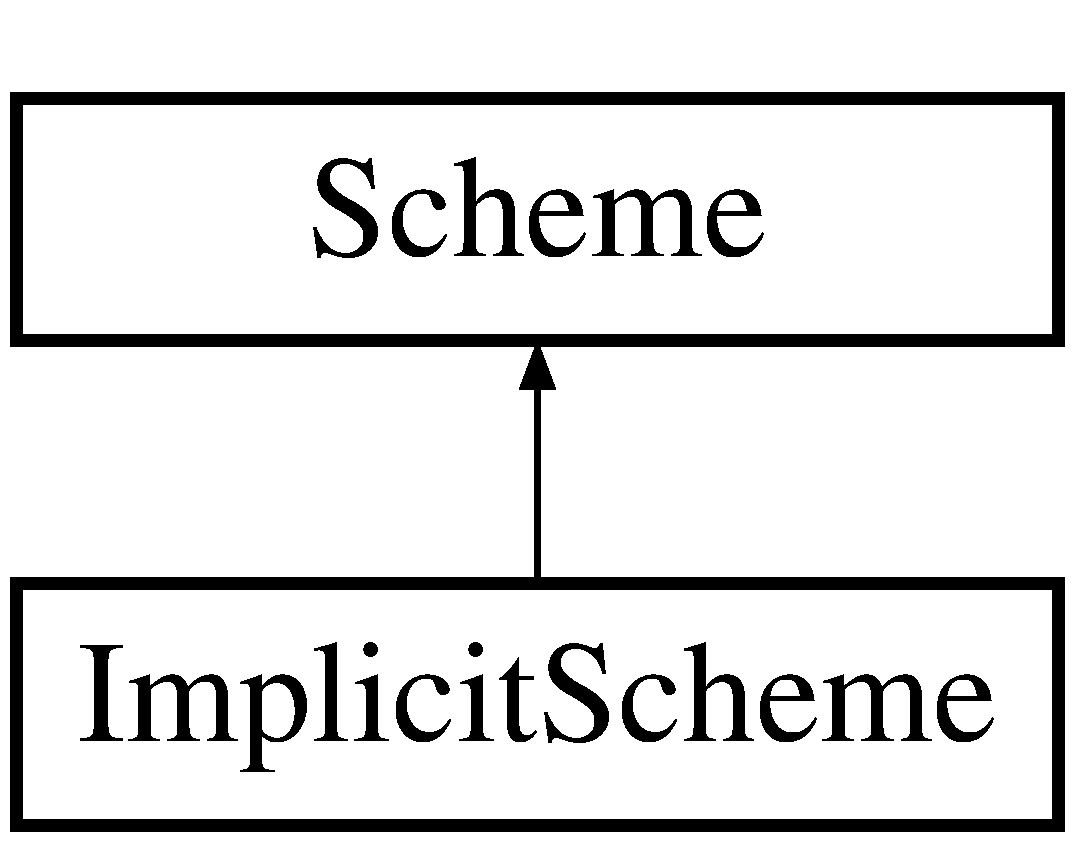
\includegraphics[height=2.000000cm]{class_implicit_scheme}
\end{center}
\end{figure}
\subsection*{Public Member Functions}
\begin{DoxyCompactItemize}
\item 
\mbox{\hyperlink{class_implicit_scheme_a7bb3a64ab8d7ca0b58ed4ba9817b8c12}{Implicit\+Scheme}} ()
\item 
string \mbox{\hyperlink{class_implicit_scheme_ab8311a005d69690622e0ddaa0dcff94d}{Implicit\+Up\+Wind\+F\+T\+BS}} ()
\item 
string \mbox{\hyperlink{class_implicit_scheme_afd2b8e73e914a04c326b8cba0d5810ce}{Implicit\+F\+T\+CS}} ()
\item 
\mbox{\hyperlink{class_implicit_scheme_aca61347d2335e248678f7f3060785762}{$\sim$\+Implicit\+Scheme}} ()
\end{DoxyCompactItemize}
\subsection*{Private Member Functions}
\begin{DoxyCompactItemize}
\item 
vector$<$ double $>$ \mbox{\hyperlink{class_implicit_scheme_a2f0cee270b60bc42f8f5e864255f5e29}{Thomas\+Algorithm}} (double parameter, double parameter2, bool version)
\end{DoxyCompactItemize}
\subsection*{Private Attributes}
\begin{DoxyCompactItemize}
\item 
vector$<$ double $>$ \mbox{\hyperlink{class_implicit_scheme_a9bd3d0a458683f9a17e8d11016c9f879}{A}}
\item 
vector$<$ double $>$ \mbox{\hyperlink{class_implicit_scheme_affeedb3fe9f7ebb8be113c884dd09a97}{B}}
\item 
vector$<$ double $>$ \mbox{\hyperlink{class_implicit_scheme_ab9059b52250e0afdd41b855299e6cf71}{C}}
\item 
vector$<$ double $>$ \mbox{\hyperlink{class_implicit_scheme_a30dad74ec599966b5ba7965f382d28cb}{D}}
\end{DoxyCompactItemize}
\subsection*{Additional Inherited Members}


\subsection{Detailed Description}
Inherited class, which includes implicit schemes like Up Wind Forward-\/\+Time Backward-\/\+Space and Forward-\/\+Time Central-\/\+Space. Additionally, class includes private method with Thomas Algorithm. 

\subsection{Constructor \& Destructor Documentation}
\mbox{\Hypertarget{class_implicit_scheme_a7bb3a64ab8d7ca0b58ed4ba9817b8c12}\label{class_implicit_scheme_a7bb3a64ab8d7ca0b58ed4ba9817b8c12}} 
\index{Implicit\+Scheme@{Implicit\+Scheme}!Implicit\+Scheme@{Implicit\+Scheme}}
\index{Implicit\+Scheme@{Implicit\+Scheme}!Implicit\+Scheme@{Implicit\+Scheme}}
\subsubsection{\texorpdfstring{Implicit\+Scheme()}{ImplicitScheme()}}
{\footnotesize\ttfamily Implicit\+Scheme\+::\+Implicit\+Scheme (\begin{DoxyParamCaption}{ }\end{DoxyParamCaption})}

Default, empty constructor for \mbox{\hyperlink{class_implicit_scheme}{Implicit\+Scheme}} class. \mbox{\Hypertarget{class_implicit_scheme_aca61347d2335e248678f7f3060785762}\label{class_implicit_scheme_aca61347d2335e248678f7f3060785762}} 
\index{Implicit\+Scheme@{Implicit\+Scheme}!````~Implicit\+Scheme@{$\sim$\+Implicit\+Scheme}}
\index{````~Implicit\+Scheme@{$\sim$\+Implicit\+Scheme}!Implicit\+Scheme@{Implicit\+Scheme}}
\subsubsection{\texorpdfstring{$\sim$\+Implicit\+Scheme()}{~ImplicitScheme()}}
{\footnotesize\ttfamily Implicit\+Scheme\+::$\sim$\+Implicit\+Scheme (\begin{DoxyParamCaption}{ }\end{DoxyParamCaption})}

Default, empty destructor for \mbox{\hyperlink{class_implicit_scheme}{Implicit\+Scheme}} class. 

\subsection{Member Function Documentation}
\mbox{\Hypertarget{class_implicit_scheme_afd2b8e73e914a04c326b8cba0d5810ce}\label{class_implicit_scheme_afd2b8e73e914a04c326b8cba0d5810ce}} 
\index{Implicit\+Scheme@{Implicit\+Scheme}!Implicit\+F\+T\+CS@{Implicit\+F\+T\+CS}}
\index{Implicit\+F\+T\+CS@{Implicit\+F\+T\+CS}!Implicit\+Scheme@{Implicit\+Scheme}}
\subsubsection{\texorpdfstring{Implicit\+F\+T\+C\+S()}{ImplicitFTCS()}}
{\footnotesize\ttfamily string Implicit\+Scheme\+::\+Implicit\+F\+T\+CS (\begin{DoxyParamCaption}{ }\end{DoxyParamCaption})}

Public method, which solves the difference using implicit scheme Forward-\/\+Time Central-\/\+Space \begin{DoxyReturn}{Returns}
string -\/ name of method for saving result into files with proper name 
\end{DoxyReturn}
\begin{DoxySeeAlso}{See also}
\mbox{\hyperlink{class_scheme_ae4512b4c8ead4d8ced95174f0b241f8a}{Save\+Result\+Into\+Files(double delta\+T, string scheme\+Name)}} 
\end{DoxySeeAlso}
\mbox{\Hypertarget{class_implicit_scheme_ab8311a005d69690622e0ddaa0dcff94d}\label{class_implicit_scheme_ab8311a005d69690622e0ddaa0dcff94d}} 
\index{Implicit\+Scheme@{Implicit\+Scheme}!Implicit\+Up\+Wind\+F\+T\+BS@{Implicit\+Up\+Wind\+F\+T\+BS}}
\index{Implicit\+Up\+Wind\+F\+T\+BS@{Implicit\+Up\+Wind\+F\+T\+BS}!Implicit\+Scheme@{Implicit\+Scheme}}
\subsubsection{\texorpdfstring{Implicit\+Up\+Wind\+F\+T\+B\+S()}{ImplicitUpWindFTBS()}}
{\footnotesize\ttfamily string Implicit\+Scheme\+::\+Implicit\+Up\+Wind\+F\+T\+BS (\begin{DoxyParamCaption}{ }\end{DoxyParamCaption})}

Public method, which solves the difference using implicit scheme Forward-\/\+Time Backward-\/\+Space \begin{DoxyReturn}{Returns}
string -\/ name of method for saving result into files with proper name 
\end{DoxyReturn}
\begin{DoxySeeAlso}{See also}
\mbox{\hyperlink{class_scheme_ae4512b4c8ead4d8ced95174f0b241f8a}{Save\+Result\+Into\+Files(double delta\+T, string scheme\+Name)}} 
\end{DoxySeeAlso}
\mbox{\Hypertarget{class_implicit_scheme_a2f0cee270b60bc42f8f5e864255f5e29}\label{class_implicit_scheme_a2f0cee270b60bc42f8f5e864255f5e29}} 
\index{Implicit\+Scheme@{Implicit\+Scheme}!Thomas\+Algorithm@{Thomas\+Algorithm}}
\index{Thomas\+Algorithm@{Thomas\+Algorithm}!Implicit\+Scheme@{Implicit\+Scheme}}
\subsubsection{\texorpdfstring{Thomas\+Algorithm()}{ThomasAlgorithm()}}
{\footnotesize\ttfamily vector$<$ double $>$ Implicit\+Scheme\+::\+Thomas\+Algorithm (\begin{DoxyParamCaption}\item[{double}]{parameter,  }\item[{double}]{parameter2,  }\item[{bool}]{version }\end{DoxyParamCaption})\hspace{0.3cm}{\ttfamily [private]}}

Private method, which includes Thomas algorithm important for Implicit schemes. \begin{DoxySeeAlso}{See also}
\mbox{\hyperlink{class_implicit_scheme_ab8311a005d69690622e0ddaa0dcff94d}{Implicit\+Up\+Wind\+F\+T\+B\+S()}} 

\mbox{\hyperlink{class_implicit_scheme_afd2b8e73e914a04c326b8cba0d5810ce}{Implicit\+F\+T\+C\+S()}} 
\end{DoxySeeAlso}
\begin{DoxyReturn}{Returns}
vector$<$double$>$ 
\end{DoxyReturn}


\subsection{Member Data Documentation}
\mbox{\Hypertarget{class_implicit_scheme_a9bd3d0a458683f9a17e8d11016c9f879}\label{class_implicit_scheme_a9bd3d0a458683f9a17e8d11016c9f879}} 
\index{Implicit\+Scheme@{Implicit\+Scheme}!A@{A}}
\index{A@{A}!Implicit\+Scheme@{Implicit\+Scheme}}
\subsubsection{\texorpdfstring{A}{A}}
{\footnotesize\ttfamily vector$<$double$>$ Implicit\+Scheme\+::A\hspace{0.3cm}{\ttfamily [private]}}

Private vector of double imortant for Thomas algorithm. \mbox{\Hypertarget{class_implicit_scheme_affeedb3fe9f7ebb8be113c884dd09a97}\label{class_implicit_scheme_affeedb3fe9f7ebb8be113c884dd09a97}} 
\index{Implicit\+Scheme@{Implicit\+Scheme}!B@{B}}
\index{B@{B}!Implicit\+Scheme@{Implicit\+Scheme}}
\subsubsection{\texorpdfstring{B}{B}}
{\footnotesize\ttfamily vector$<$double$>$ Implicit\+Scheme\+::B\hspace{0.3cm}{\ttfamily [private]}}

Private vector of double imortant for Thomas algorithm. \mbox{\Hypertarget{class_implicit_scheme_ab9059b52250e0afdd41b855299e6cf71}\label{class_implicit_scheme_ab9059b52250e0afdd41b855299e6cf71}} 
\index{Implicit\+Scheme@{Implicit\+Scheme}!C@{C}}
\index{C@{C}!Implicit\+Scheme@{Implicit\+Scheme}}
\subsubsection{\texorpdfstring{C}{C}}
{\footnotesize\ttfamily vector$<$double$>$ Implicit\+Scheme\+::C\hspace{0.3cm}{\ttfamily [private]}}

Private vector of double imortant for Thomas algorithm. \mbox{\Hypertarget{class_implicit_scheme_a30dad74ec599966b5ba7965f382d28cb}\label{class_implicit_scheme_a30dad74ec599966b5ba7965f382d28cb}} 
\index{Implicit\+Scheme@{Implicit\+Scheme}!D@{D}}
\index{D@{D}!Implicit\+Scheme@{Implicit\+Scheme}}
\subsubsection{\texorpdfstring{D}{D}}
{\footnotesize\ttfamily vector$<$double$>$ Implicit\+Scheme\+::D\hspace{0.3cm}{\ttfamily [private]}}

Private vector of double imortant for Thomas algorithm. 

The documentation for this class was generated from the following files\+:\begin{DoxyCompactItemize}
\item 
\mbox{\hyperlink{_implicit_scheme_8h}{Implicit\+Scheme.\+h}}\item 
\mbox{\hyperlink{_implicit_scheme_8cpp}{Implicit\+Scheme.\+cpp}}\end{DoxyCompactItemize}

\hypertarget{class_matrix}{}\section{Matrix Class Reference}
\label{class_matrix}\index{Matrix@{Matrix}}


{\ttfamily \#include $<$matrix.\+h$>$}

Inheritance diagram for Matrix\+:\begin{figure}[H]
\begin{center}
\leavevmode
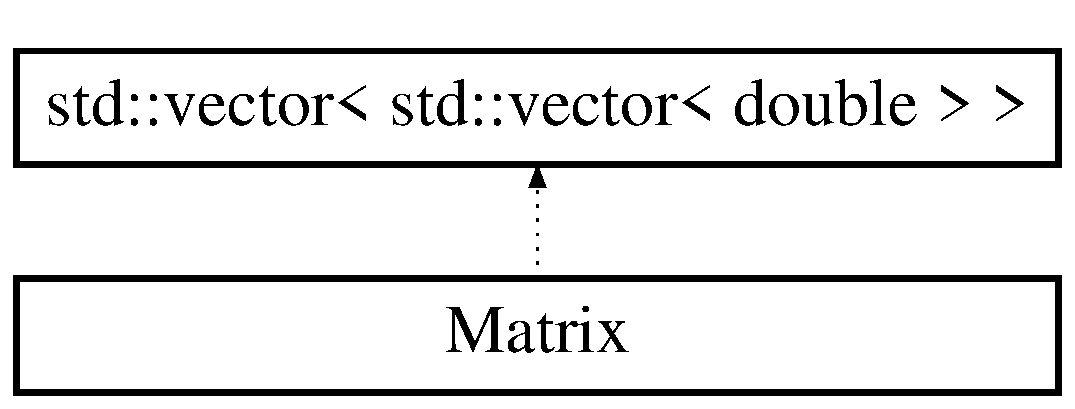
\includegraphics[height=2.000000cm]{class_matrix}
\end{center}
\end{figure}
\subsection*{Public Member Functions}
\begin{DoxyCompactItemize}
\item 
\mbox{\hyperlink{class_matrix_a2dba13c45127354c9f75ef576f49269b}{Matrix}} ()
\item 
\mbox{\hyperlink{class_matrix_a135a15de1126d735bb95fcc839d739d7}{Matrix}} (int Nrows, int Ncols)
\item 
\mbox{\hyperlink{class_matrix_a765f4dcb51b6829311cc3e7576388423}{Matrix}} (const \mbox{\hyperlink{class_matrix}{Matrix}} \&m)
\item 
int \mbox{\hyperlink{class_matrix_a711f84a1c62832d9d197d78c9855a276}{get\+Nrows}} () const
\item 
int \mbox{\hyperlink{class_matrix_ae0a5f2154953b8d129a90b04f91d9079}{get\+Ncols}} () const
\item 
\mbox{\hyperlink{class_matrix}{Matrix}} \& \mbox{\hyperlink{class_matrix_aea5a06385f646eb4a63929fae6fa3e14}{operator=}} (const \mbox{\hyperlink{class_matrix}{Matrix}} \&m)
\item 
bool \mbox{\hyperlink{class_matrix_a35097c20bcb1495b57d452db0d7b1f53}{operator==}} (const \mbox{\hyperlink{class_matrix}{Matrix}} \&m) const
\item 
\mbox{\hyperlink{class_matrix}{Matrix}} \mbox{\hyperlink{class_matrix_a2aabf841a4302d528f8b102c0800a263}{operator-\/}} (\mbox{\hyperlink{class_matrix}{Matrix}} m)
\item 
double \mbox{\hyperlink{class_matrix_af4d468252f3ecbbcaa5726c76e332b4c}{one\+\_\+norm}} () const
\item 
double \mbox{\hyperlink{class_matrix_aac496af05ec7aa26afc2b9c6d0ab8b66}{two\+\_\+norm}} () const
\item 
double \mbox{\hyperlink{class_matrix_a43066c7fe6418aad40170b85415063e8}{uniform\+\_\+norm}} () const
\item 
\mbox{\hyperlink{class_matrix}{Matrix}} \mbox{\hyperlink{class_matrix_aaa40c78e6b3bb5bbf572d35612dbf6a7}{operator$\ast$}} (const \mbox{\hyperlink{class_matrix}{Matrix}} \&a) const
\item 
\mbox{\hyperlink{class_matrix}{Matrix}} \mbox{\hyperlink{class_matrix_a759661b75b9681f3a89ff75e27933b3a}{transpose}} () const
\end{DoxyCompactItemize}
\subsection*{Friends}
\begin{DoxyCompactItemize}
\item 
std\+::istream \& \mbox{\hyperlink{class_matrix_a3d6c1dcfc038804f4c08687f4f37f48b}{operator$>$$>$}} (std\+::istream \&is, \mbox{\hyperlink{class_matrix}{Matrix}} \&m)
\item 
std\+::ostream \& \mbox{\hyperlink{class_matrix_a060711074cb5bcaf4e75498bc040c4b7}{operator$<$$<$}} (std\+::ostream \&os, const \mbox{\hyperlink{class_matrix}{Matrix}} \&m)
\item 
std\+::ifstream \& \mbox{\hyperlink{class_matrix_aa5699a0bdf0ee014f083ff8a76629d21}{operator$>$$>$}} (std\+::ifstream \&ifs, \mbox{\hyperlink{class_matrix}{Matrix}} \&m)
\item 
std\+::ofstream \& \mbox{\hyperlink{class_matrix_aa574249d63b390cf1108d6e82047ef61}{operator$<$$<$}} (std\+::ofstream \&ofs, const \mbox{\hyperlink{class_matrix}{Matrix}} \&m)
\end{DoxyCompactItemize}


\subsection{Detailed Description}
\mbox{\hyperlink{class_matrix}{Matrix}} class, which use vector container for Standard Template Library. Important class for \mbox{\hyperlink{class_scheme}{Scheme}}, \mbox{\hyperlink{class_explicit_scheme}{Explicit\+Scheme}} and \mbox{\hyperlink{class_implicit_scheme}{Implicit\+Scheme}} classes. 

\subsection{Constructor \& Destructor Documentation}
\mbox{\Hypertarget{class_matrix_a2dba13c45127354c9f75ef576f49269b}\label{class_matrix_a2dba13c45127354c9f75ef576f49269b}} 
\index{Matrix@{Matrix}!Matrix@{Matrix}}
\index{Matrix@{Matrix}!Matrix@{Matrix}}
\subsubsection{\texorpdfstring{Matrix()}{Matrix()}\hspace{0.1cm}{\footnotesize\ttfamily [1/3]}}
{\footnotesize\ttfamily Matrix\+::\+Matrix (\begin{DoxyParamCaption}{ }\end{DoxyParamCaption})}

Default constructor. Intialize an empty \mbox{\hyperlink{class_matrix}{Matrix}} object \begin{DoxySeeAlso}{See also}
\mbox{\hyperlink{class_matrix_a135a15de1126d735bb95fcc839d739d7}{Matrix(int Nrows, int Ncols)}} 

\mbox{\hyperlink{class_matrix_a765f4dcb51b6829311cc3e7576388423}{Matrix(const Matrix\& m)}} 
\end{DoxySeeAlso}
\mbox{\Hypertarget{class_matrix_a135a15de1126d735bb95fcc839d739d7}\label{class_matrix_a135a15de1126d735bb95fcc839d739d7}} 
\index{Matrix@{Matrix}!Matrix@{Matrix}}
\index{Matrix@{Matrix}!Matrix@{Matrix}}
\subsubsection{\texorpdfstring{Matrix()}{Matrix()}\hspace{0.1cm}{\footnotesize\ttfamily [2/3]}}
{\footnotesize\ttfamily Matrix\+::\+Matrix (\begin{DoxyParamCaption}\item[{int}]{Nrows,  }\item[{int}]{Ncols }\end{DoxyParamCaption})}

Alternate constructor. build a matrix Nrows by Ncols \begin{DoxySeeAlso}{See also}
\mbox{\hyperlink{class_matrix_a2dba13c45127354c9f75ef576f49269b}{Matrix()}} 

\mbox{\hyperlink{class_matrix_a765f4dcb51b6829311cc3e7576388423}{Matrix(const Matrix\& m)}} 
\end{DoxySeeAlso}

\begin{DoxyExceptions}{Exceptions}
{\em invalid\+\_\+argument} & (\char`\"{}matrix size negative or zero\char`\"{}) \\
\hline
\end{DoxyExceptions}

\begin{DoxyParams}{Parameters}
{\em Nrows} & int. number of rows in matrix \\
\hline
{\em Ncols} & int. number of columns in matrix \\
\hline
\end{DoxyParams}
\mbox{\Hypertarget{class_matrix_a765f4dcb51b6829311cc3e7576388423}\label{class_matrix_a765f4dcb51b6829311cc3e7576388423}} 
\index{Matrix@{Matrix}!Matrix@{Matrix}}
\index{Matrix@{Matrix}!Matrix@{Matrix}}
\subsubsection{\texorpdfstring{Matrix()}{Matrix()}\hspace{0.1cm}{\footnotesize\ttfamily [3/3]}}
{\footnotesize\ttfamily Matrix\+::\+Matrix (\begin{DoxyParamCaption}\item[{const \mbox{\hyperlink{class_matrix}{Matrix}} \&}]{m }\end{DoxyParamCaption})}

Copy constructor. build a matrix from another matrix \begin{DoxySeeAlso}{See also}
\mbox{\hyperlink{class_matrix_a2dba13c45127354c9f75ef576f49269b}{Matrix()}} 

\mbox{\hyperlink{class_matrix_a135a15de1126d735bb95fcc839d739d7}{Matrix(int Nrows, int Ncols)}} 
\end{DoxySeeAlso}

\begin{DoxyParams}{Parameters}
{\em m} & \mbox{\hyperlink{class_matrix}{Matrix}}\&. matrix to copy from \\
\hline
\end{DoxyParams}


\subsection{Member Function Documentation}
\mbox{\Hypertarget{class_matrix_ae0a5f2154953b8d129a90b04f91d9079}\label{class_matrix_ae0a5f2154953b8d129a90b04f91d9079}} 
\index{Matrix@{Matrix}!get\+Ncols@{get\+Ncols}}
\index{get\+Ncols@{get\+Ncols}!Matrix@{Matrix}}
\subsubsection{\texorpdfstring{get\+Ncols()}{getNcols()}}
{\footnotesize\ttfamily int Matrix\+::get\+Ncols (\begin{DoxyParamCaption}{ }\end{DoxyParamCaption}) const}

Normal public get method. get the number of columns \begin{DoxySeeAlso}{See also}
int \mbox{\hyperlink{class_matrix_a711f84a1c62832d9d197d78c9855a276}{get\+Nrows()const}} 
\end{DoxySeeAlso}
\begin{DoxyReturn}{Returns}
int. number of columns in matrix 
\end{DoxyReturn}
\mbox{\Hypertarget{class_matrix_a711f84a1c62832d9d197d78c9855a276}\label{class_matrix_a711f84a1c62832d9d197d78c9855a276}} 
\index{Matrix@{Matrix}!get\+Nrows@{get\+Nrows}}
\index{get\+Nrows@{get\+Nrows}!Matrix@{Matrix}}
\subsubsection{\texorpdfstring{get\+Nrows()}{getNrows()}}
{\footnotesize\ttfamily int Matrix\+::get\+Nrows (\begin{DoxyParamCaption}{ }\end{DoxyParamCaption}) const}

Normal public get method. get the number of rows \begin{DoxySeeAlso}{See also}
int \mbox{\hyperlink{class_matrix_ae0a5f2154953b8d129a90b04f91d9079}{get\+Ncols()const}} 
\end{DoxySeeAlso}
\begin{DoxyReturn}{Returns}
int. number of rows in matrix 
\end{DoxyReturn}
\mbox{\Hypertarget{class_matrix_af4d468252f3ecbbcaa5726c76e332b4c}\label{class_matrix_af4d468252f3ecbbcaa5726c76e332b4c}} 
\index{Matrix@{Matrix}!one\+\_\+norm@{one\+\_\+norm}}
\index{one\+\_\+norm@{one\+\_\+norm}!Matrix@{Matrix}}
\subsubsection{\texorpdfstring{one\+\_\+norm()}{one\_norm()}}
{\footnotesize\ttfamily double Matrix\+::one\+\_\+norm (\begin{DoxyParamCaption}{ }\end{DoxyParamCaption}) const}

Normal public method that returns a double. It returns L1 norm of matrix \begin{DoxySeeAlso}{See also}
\mbox{\hyperlink{class_matrix_aac496af05ec7aa26afc2b9c6d0ab8b66}{two\+\_\+norm()const}} 

\mbox{\hyperlink{class_matrix_a43066c7fe6418aad40170b85415063e8}{uniform\+\_\+norm()const}} 
\end{DoxySeeAlso}
\begin{DoxyReturn}{Returns}
double. matrix L1 norm 
\end{DoxyReturn}
\mbox{\Hypertarget{class_matrix_aaa40c78e6b3bb5bbf572d35612dbf6a7}\label{class_matrix_aaa40c78e6b3bb5bbf572d35612dbf6a7}} 
\index{Matrix@{Matrix}!operator$\ast$@{operator$\ast$}}
\index{operator$\ast$@{operator$\ast$}!Matrix@{Matrix}}
\subsubsection{\texorpdfstring{operator$\ast$()}{operator*()}}
{\footnotesize\ttfamily \mbox{\hyperlink{class_matrix}{Matrix}} Matrix\+::operator$\ast$ (\begin{DoxyParamCaption}\item[{const \mbox{\hyperlink{class_matrix}{Matrix}} \&}]{a }\end{DoxyParamCaption}) const}

Overloaded $\ast$operator that returns a \mbox{\hyperlink{class_matrix}{Matrix}}. It Performs matrix by matrix multiplication. \begin{DoxySeeAlso}{See also}
\mbox{\hyperlink{class_matrix_aaa40c78e6b3bb5bbf572d35612dbf6a7}{operator$\ast$(const Matrix \& a) const}} 
\end{DoxySeeAlso}

\begin{DoxyExceptions}{Exceptions}
{\em out\+\_\+of\+\_\+range} & (\char`\"{}\+Matrix access error\char`\"{}) One or more of the matrix have a zero size \\
\hline
{\em std\+::out\+\_\+of\+\_\+range} & (\char`\"{}uncompatible matrix sizes\char`\"{}) Number of columns in first matrix do not match number of columns in second matrix \\
\hline
\end{DoxyExceptions}
\begin{DoxyReturn}{Returns}
\mbox{\hyperlink{class_matrix}{Matrix}}. matrix-\/matrix product 
\end{DoxyReturn}

\begin{DoxyParams}{Parameters}
{\em a} & \mbox{\hyperlink{class_matrix}{Matrix}}. matrix to multiply by \\
\hline
\end{DoxyParams}
\mbox{\Hypertarget{class_matrix_a2aabf841a4302d528f8b102c0800a263}\label{class_matrix_a2aabf841a4302d528f8b102c0800a263}} 
\index{Matrix@{Matrix}!operator-\/@{operator-\/}}
\index{operator-\/@{operator-\/}!Matrix@{Matrix}}
\subsubsection{\texorpdfstring{operator-\/()}{operator-()}}
{\footnotesize\ttfamily \mbox{\hyperlink{class_matrix}{Matrix}} Matrix\+::operator-\/ (\begin{DoxyParamCaption}\item[{\mbox{\hyperlink{class_matrix}{Matrix}}}]{m }\end{DoxyParamCaption})}

Overloaded subtraction operator returns \mbox{\hyperlink{class_matrix}{Matrix}} \begin{DoxySeeAlso}{See also}
\mbox{\hyperlink{class_matrix_a2aabf841a4302d528f8b102c0800a263}{operator-\/(\+Matrix m)}} 
\end{DoxySeeAlso}
\begin{DoxyReturn}{Returns}
\mbox{\hyperlink{class_matrix}{Matrix}} 
\end{DoxyReturn}
\mbox{\Hypertarget{class_matrix_aea5a06385f646eb4a63929fae6fa3e14}\label{class_matrix_aea5a06385f646eb4a63929fae6fa3e14}} 
\index{Matrix@{Matrix}!operator=@{operator=}}
\index{operator=@{operator=}!Matrix@{Matrix}}
\subsubsection{\texorpdfstring{operator=()}{operator=()}}
{\footnotesize\ttfamily \mbox{\hyperlink{class_matrix}{Matrix}} \& Matrix\+::operator= (\begin{DoxyParamCaption}\item[{const \mbox{\hyperlink{class_matrix}{Matrix}} \&}]{m }\end{DoxyParamCaption})}

Overloaded assignment operator \begin{DoxySeeAlso}{See also}
\mbox{\hyperlink{class_matrix_a35097c20bcb1495b57d452db0d7b1f53}{operator==(const Matrix\& m)const}} 
\end{DoxySeeAlso}
\begin{DoxyReturn}{Returns}
\mbox{\hyperlink{class_matrix}{Matrix}}\&. the matrix on the left of the assignment 
\end{DoxyReturn}

\begin{DoxyParams}{Parameters}
{\em m} & \mbox{\hyperlink{class_matrix}{Matrix}}\&. \mbox{\hyperlink{class_matrix}{Matrix}} to assign from \\
\hline
\end{DoxyParams}
\mbox{\Hypertarget{class_matrix_a35097c20bcb1495b57d452db0d7b1f53}\label{class_matrix_a35097c20bcb1495b57d452db0d7b1f53}} 
\index{Matrix@{Matrix}!operator==@{operator==}}
\index{operator==@{operator==}!Matrix@{Matrix}}
\subsubsection{\texorpdfstring{operator==()}{operator==()}}
{\footnotesize\ttfamily bool Matrix\+::operator== (\begin{DoxyParamCaption}\item[{const \mbox{\hyperlink{class_matrix}{Matrix}} \&}]{m }\end{DoxyParamCaption}) const}

Overloaded comparison operator returns true or false depending on whether the matrices are the same or not \begin{DoxySeeAlso}{See also}
\mbox{\hyperlink{class_matrix_aea5a06385f646eb4a63929fae6fa3e14}{operator=(const Matrix\& m)}} 
\end{DoxySeeAlso}
\begin{DoxyReturn}{Returns}
bool. true or false 
\end{DoxyReturn}

\begin{DoxyParams}{Parameters}
{\em m} & \mbox{\hyperlink{class_matrix}{Matrix}}\&. \mbox{\hyperlink{class_matrix}{Matrix}} to compare to \\
\hline
\end{DoxyParams}
\mbox{\Hypertarget{class_matrix_a759661b75b9681f3a89ff75e27933b3a}\label{class_matrix_a759661b75b9681f3a89ff75e27933b3a}} 
\index{Matrix@{Matrix}!transpose@{transpose}}
\index{transpose@{transpose}!Matrix@{Matrix}}
\subsubsection{\texorpdfstring{transpose()}{transpose()}}
{\footnotesize\ttfamily \mbox{\hyperlink{class_matrix}{Matrix}} Matrix\+::transpose (\begin{DoxyParamCaption}{ }\end{DoxyParamCaption}) const}

public method that returns the transpose of the matrix. It returns the transpose of matrix \begin{DoxyReturn}{Returns}
\mbox{\hyperlink{class_matrix}{Matrix}}. matrix transpose 
\end{DoxyReturn}
\mbox{\Hypertarget{class_matrix_aac496af05ec7aa26afc2b9c6d0ab8b66}\label{class_matrix_aac496af05ec7aa26afc2b9c6d0ab8b66}} 
\index{Matrix@{Matrix}!two\+\_\+norm@{two\+\_\+norm}}
\index{two\+\_\+norm@{two\+\_\+norm}!Matrix@{Matrix}}
\subsubsection{\texorpdfstring{two\+\_\+norm()}{two\_norm()}}
{\footnotesize\ttfamily double Matrix\+::two\+\_\+norm (\begin{DoxyParamCaption}{ }\end{DoxyParamCaption}) const}

Normal public method that returns a double. It returns L2 norm of matrix \begin{DoxySeeAlso}{See also}
\mbox{\hyperlink{class_matrix_af4d468252f3ecbbcaa5726c76e332b4c}{one\+\_\+norm()const}} 

\mbox{\hyperlink{class_matrix_a43066c7fe6418aad40170b85415063e8}{uniform\+\_\+norm()const}} 
\end{DoxySeeAlso}
\begin{DoxyReturn}{Returns}
double. matrix L2 norm 
\end{DoxyReturn}
\mbox{\Hypertarget{class_matrix_a43066c7fe6418aad40170b85415063e8}\label{class_matrix_a43066c7fe6418aad40170b85415063e8}} 
\index{Matrix@{Matrix}!uniform\+\_\+norm@{uniform\+\_\+norm}}
\index{uniform\+\_\+norm@{uniform\+\_\+norm}!Matrix@{Matrix}}
\subsubsection{\texorpdfstring{uniform\+\_\+norm()}{uniform\_norm()}}
{\footnotesize\ttfamily double Matrix\+::uniform\+\_\+norm (\begin{DoxyParamCaption}{ }\end{DoxyParamCaption}) const}

Normal public method that returns a double. It returns L\+\_\+max norm of matrix \begin{DoxySeeAlso}{See also}
\mbox{\hyperlink{class_matrix_af4d468252f3ecbbcaa5726c76e332b4c}{one\+\_\+norm()const}} 

\mbox{\hyperlink{class_matrix_aac496af05ec7aa26afc2b9c6d0ab8b66}{two\+\_\+norm()const}} 
\end{DoxySeeAlso}
\begin{DoxyReturn}{Returns}
double. matrix L\+\_\+max norm 
\end{DoxyReturn}


\subsection{Friends And Related Function Documentation}
\mbox{\Hypertarget{class_matrix_a060711074cb5bcaf4e75498bc040c4b7}\label{class_matrix_a060711074cb5bcaf4e75498bc040c4b7}} 
\index{Matrix@{Matrix}!operator$<$$<$@{operator$<$$<$}}
\index{operator$<$$<$@{operator$<$$<$}!Matrix@{Matrix}}
\subsubsection{\texorpdfstring{operator$<$$<$}{operator<<}\hspace{0.1cm}{\footnotesize\ttfamily [1/2]}}
{\footnotesize\ttfamily std\+::ostream\& operator$<$$<$ (\begin{DoxyParamCaption}\item[{std\+::ostream \&}]{os,  }\item[{const \mbox{\hyperlink{class_matrix}{Matrix}} \&}]{m }\end{DoxyParamCaption})\hspace{0.3cm}{\ttfamily [friend]}}

Overloaded ostream $<$$<$ operator. Display output if matrix has size user will be asked to input only matrix values if matrix was not initialized user can choose matrix size and input it values \begin{DoxySeeAlso}{See also}
\mbox{\hyperlink{class_matrix_aa5699a0bdf0ee014f083ff8a76629d21}{operator$>$$>$(std\+::ifstream\& ifs, Matrix\& m)}} 

\mbox{\hyperlink{class_matrix_a3d6c1dcfc038804f4c08687f4f37f48b}{operator$>$$>$(std\+::istream\& is, Matrix\& m)}} 

\mbox{\hyperlink{class_matrix_a060711074cb5bcaf4e75498bc040c4b7}{operator$<$$<$(std\+::ostream\& os, const Matrix\& m)}} 
\end{DoxySeeAlso}
\begin{DoxyReturn}{Returns}
std\+::ostream\&. The ostream object 
\end{DoxyReturn}

\begin{DoxyParams}{Parameters}
{\em os} & Display output stream \\
\hline
{\em m} & \mbox{\hyperlink{class_matrix}{Matrix}} to read from \\
\hline
\end{DoxyParams}
\mbox{\Hypertarget{class_matrix_aa574249d63b390cf1108d6e82047ef61}\label{class_matrix_aa574249d63b390cf1108d6e82047ef61}} 
\index{Matrix@{Matrix}!operator$<$$<$@{operator$<$$<$}}
\index{operator$<$$<$@{operator$<$$<$}!Matrix@{Matrix}}
\subsubsection{\texorpdfstring{operator$<$$<$}{operator<<}\hspace{0.1cm}{\footnotesize\ttfamily [2/2]}}
{\footnotesize\ttfamily std\+::ofstream\& operator$<$$<$ (\begin{DoxyParamCaption}\item[{std\+::ofstream \&}]{ofs,  }\item[{const \mbox{\hyperlink{class_matrix}{Matrix}} \&}]{m }\end{DoxyParamCaption})\hspace{0.3cm}{\ttfamily [friend]}}

Overloaded ofstream $<$$<$ operator. File output the file output operator is compatible with file input operator, ie. everything written can be read later. \begin{DoxySeeAlso}{See also}
\mbox{\hyperlink{class_matrix_aa5699a0bdf0ee014f083ff8a76629d21}{operator$>$$>$(std\+::ifstream\& ifs, Matrix\& m)}} 

\mbox{\hyperlink{class_matrix_aa574249d63b390cf1108d6e82047ef61}{operator$<$$<$(std\+::ofstream\& ofs, const Matrix\& m)}} 

\mbox{\hyperlink{class_matrix_a3d6c1dcfc038804f4c08687f4f37f48b}{operator$>$$>$(std\+::istream\& is, Matrix\& m)}} 
\end{DoxySeeAlso}

\begin{DoxyExceptions}{Exceptions}
{\em std\+::invalid\+\_\+argument} & (\char`\"{}file read error -\/ negative matrix size\char`\"{}); \\
\hline
\end{DoxyExceptions}
\begin{DoxyReturn}{Returns}
std\+::ofstream\&. The ofstream object 
\end{DoxyReturn}

\begin{DoxyParams}{Parameters}
{\em m} & \mbox{\hyperlink{class_matrix}{Matrix}} to read from \\
\hline
\end{DoxyParams}
\mbox{\Hypertarget{class_matrix_a3d6c1dcfc038804f4c08687f4f37f48b}\label{class_matrix_a3d6c1dcfc038804f4c08687f4f37f48b}} 
\index{Matrix@{Matrix}!operator$>$$>$@{operator$>$$>$}}
\index{operator$>$$>$@{operator$>$$>$}!Matrix@{Matrix}}
\subsubsection{\texorpdfstring{operator$>$$>$}{operator>>}\hspace{0.1cm}{\footnotesize\ttfamily [1/2]}}
{\footnotesize\ttfamily std\+::istream\& operator$>$$>$ (\begin{DoxyParamCaption}\item[{std\+::istream \&}]{is,  }\item[{\mbox{\hyperlink{class_matrix}{Matrix}} \&}]{m }\end{DoxyParamCaption})\hspace{0.3cm}{\ttfamily [friend]}}

Overloaded istream $>$$>$ operator. Keyboard input if matrix has size user will be asked to input only matrix values if matrix was not initialized user can choose matrix size and input it values \begin{DoxySeeAlso}{See also}
\mbox{\hyperlink{class_matrix_aa574249d63b390cf1108d6e82047ef61}{operator$<$$<$(std\+::ofstream\& ofs, const Matrix\& m)}} 

\mbox{\hyperlink{class_matrix_a3d6c1dcfc038804f4c08687f4f37f48b}{operator$>$$>$(std\+::istream\& is, Matrix\& m)}} 

\mbox{\hyperlink{class_matrix_a060711074cb5bcaf4e75498bc040c4b7}{operator$<$$<$(std\+::ostream\& os, const Matrix\& m)}} 
\end{DoxySeeAlso}

\begin{DoxyExceptions}{Exceptions}
{\em std\+::invalid\+\_\+argument} & (\char`\"{}read error -\/ negative matrix size\char`\"{}); \\
\hline
\end{DoxyExceptions}
\begin{DoxyReturn}{Returns}
std\+::istream\&. The istream object 
\end{DoxyReturn}

\begin{DoxyParams}{Parameters}
{\em is} & Keyboard input stream \\
\hline
{\em m} & \mbox{\hyperlink{class_matrix}{Matrix}} to write into \\
\hline
\end{DoxyParams}
\mbox{\Hypertarget{class_matrix_aa5699a0bdf0ee014f083ff8a76629d21}\label{class_matrix_aa5699a0bdf0ee014f083ff8a76629d21}} 
\index{Matrix@{Matrix}!operator$>$$>$@{operator$>$$>$}}
\index{operator$>$$>$@{operator$>$$>$}!Matrix@{Matrix}}
\subsubsection{\texorpdfstring{operator$>$$>$}{operator>>}\hspace{0.1cm}{\footnotesize\ttfamily [2/2]}}
{\footnotesize\ttfamily std\+::ifstream\& operator$>$$>$ (\begin{DoxyParamCaption}\item[{std\+::ifstream \&}]{ifs,  }\item[{\mbox{\hyperlink{class_matrix}{Matrix}} \&}]{m }\end{DoxyParamCaption})\hspace{0.3cm}{\ttfamily [friend]}}

Overloaded ifstream $>$$>$ operator. File input the file output operator is compatible with file input operator, ie. everything written can be read later. \begin{DoxySeeAlso}{See also}
\mbox{\hyperlink{class_matrix_aa5699a0bdf0ee014f083ff8a76629d21}{operator$>$$>$(std\+::ifstream\& ifs, Matrix\& m)}} 

\mbox{\hyperlink{class_matrix_aa574249d63b390cf1108d6e82047ef61}{operator$<$$<$(std\+::ofstream\& ofs, const Matrix\& m)}} 

\mbox{\hyperlink{class_matrix_a060711074cb5bcaf4e75498bc040c4b7}{operator$<$$<$(std\+::ostream\& os, const Matrix\& m)}} 
\end{DoxySeeAlso}
\begin{DoxyReturn}{Returns}
std\+::ifstream\&. The ifstream object 
\end{DoxyReturn}

\begin{DoxyParams}{Parameters}
{\em ifs} & Input file stream with opened matrix file \\
\hline
{\em m} & \mbox{\hyperlink{class_matrix}{Matrix}} to write into \\
\hline
\end{DoxyParams}


The documentation for this class was generated from the following files\+:\begin{DoxyCompactItemize}
\item 
\mbox{\hyperlink{matrix_8h}{matrix.\+h}}\item 
\mbox{\hyperlink{matrix_8cpp}{matrix.\+cpp}}\end{DoxyCompactItemize}

\hypertarget{class_scheme}{}\section{Scheme Class Reference}
\label{class_scheme}\index{Scheme@{Scheme}}


{\ttfamily \#include $<$Scheme.\+h$>$}



Inheritance diagram for Scheme\+:
% FIG 0


Collaboration diagram for Scheme\+:
% FIG 1
\subsection*{Public Member Functions}
\begin{DoxyCompactItemize}
\item 
\mbox{\hyperlink{class_scheme_aa0b319a6594176dea40ca78562401b53}{Scheme}} ()
\item 
void \mbox{\hyperlink{class_scheme_ae4512b4c8ead4d8ced95174f0b241f8a}{Save\+Result\+Into\+Files}} (double \mbox{\hyperlink{class_scheme_aaaf978f98d30bd96ea56a9387d1b2c5a}{deltaT}}, string scheme\+Name)
\item 
string \mbox{\hyperlink{class_scheme_a7d3e9f8133a955517471eb7a6fea355f}{Analytical\+Solution}} (double default\+DeltaT=0)
\item 
void \mbox{\hyperlink{class_scheme_ae098876d0287ac2bf5220608db2a8468}{Compute\+Norms}} (\mbox{\hyperlink{class_matrix}{Matrix}} m1, \mbox{\hyperlink{class_matrix}{Matrix}} m2)
\item 
void \mbox{\hyperlink{class_scheme_ae26048cf5128c6ea6e698a7036f2cc42}{Print\+Result}} ()
\item 
\mbox{\hyperlink{class_matrix}{Matrix}} \mbox{\hyperlink{class_scheme_a14c333d182a6b4e94aa2a346000257ea}{Get\+Matrix}} ()
\item 
double \mbox{\hyperlink{class_scheme_af05aa7671d5c080c0cca501cb6717cd0}{Get\+DeltaT}} ()
\item 
\mbox{\hyperlink{class_scheme_af8f283786d3b27d97c55d92b9ae8b20b}{$\sim$\+Scheme}} ()
\end{DoxyCompactItemize}
\subsection*{Protected Member Functions}
\begin{DoxyCompactItemize}
\item 
void \mbox{\hyperlink{class_scheme_ad3546cda995629a2792629a072760ad2}{Initial\+Condition}} ()
\item 
void \mbox{\hyperlink{class_scheme_a36885039937c25f13c8daea654e37b97}{Boundry\+Condition}} ()
\item 
void \mbox{\hyperlink{class_scheme_ac5803e4951dc125b274f543d5037c21d}{Insert\+DeltaT}} ()
\item 
void \mbox{\hyperlink{class_scheme_a0364e328d78e84be15d293a66d946008}{Compute\+Size\+Of\+Matrix}} (bool if\+Printed=1)
\end{DoxyCompactItemize}
\subsection*{Protected Attributes}
\begin{DoxyCompactItemize}
\item 
\mbox{\hyperlink{class_matrix}{Matrix}} \mbox{\hyperlink{class_scheme_a0e1fb8cb7e062d3f49715445a884f0e8}{matrix}}
\item 
int \mbox{\hyperlink{class_scheme_aaa37febfb3b695d7637210b6ffdcd9ad}{size\+Of\+Matrix}}
\item 
int \mbox{\hyperlink{class_scheme_a04f4e41aaa2bffd82b9027550f8374f0}{sizeT}}
\item 
int \mbox{\hyperlink{class_scheme_a34d6e438fa45638221f250c9aa7acde1}{sizeX}}
\item 
double \mbox{\hyperlink{class_scheme_aaaf978f98d30bd96ea56a9387d1b2c5a}{deltaT}}
\item 
double \mbox{\hyperlink{class_scheme_a7491f0ce42370ab44134bf82bd0079a7}{deltaX}}
\item 
const double \mbox{\hyperlink{class_scheme_a1a21e7fac3843f2d64c49597c668ce56}{PI}} = atan(1) $\ast$ 4
\item 
const double \mbox{\hyperlink{class_scheme_a512873bf3cd534832300046f1a1792a3}{u}} = 250
\end{DoxyCompactItemize}
\subsection*{Friends}
\begin{DoxyCompactItemize}
\item 
bool \mbox{\hyperlink{class_scheme_ad9aa7a2eac63a3a91e6efc3d8a8093cd}{Is\+Double}} (string input)
\end{DoxyCompactItemize}


\subsection{Detailed Description}
The \mbox{\hyperlink{class_scheme}{Scheme}} class is mother/core class for \mbox{\hyperlink{class_explicit_scheme}{Explicit\+Scheme}} and \mbox{\hyperlink{class_implicit_scheme}{Implicit\+Scheme}} classes. This class includes common elements for inheritance classes like\+: computing initial condition, boundry condition and others. Additionally, \mbox{\hyperlink{class_scheme}{Scheme}} class includes methods responsible for printing results in the console, saving results into text files. Objects are protected, because they can be used only in mother class and inheritance classes. Class includes only one default constructor and one default destructor. The \mbox{\hyperlink{class_scheme}{Scheme}} class includes protected and public methods. Some accessors and one friend method are available. 

\subsection{Constructor \& Destructor Documentation}
\mbox{\Hypertarget{class_scheme_aa0b319a6594176dea40ca78562401b53}\label{class_scheme_aa0b319a6594176dea40ca78562401b53}} 
\index{Scheme@{Scheme}!Scheme@{Scheme}}
\index{Scheme@{Scheme}!Scheme@{Scheme}}
\subsubsection{\texorpdfstring{Scheme()}{Scheme()}}
{\footnotesize\ttfamily Scheme\+::\+Scheme (\begin{DoxyParamCaption}{ }\end{DoxyParamCaption})}

Default, empty constructor for \mbox{\hyperlink{class_scheme}{Scheme}} class. \mbox{\Hypertarget{class_scheme_af8f283786d3b27d97c55d92b9ae8b20b}\label{class_scheme_af8f283786d3b27d97c55d92b9ae8b20b}} 
\index{Scheme@{Scheme}!````~Scheme@{$\sim$\+Scheme}}
\index{````~Scheme@{$\sim$\+Scheme}!Scheme@{Scheme}}
\subsubsection{\texorpdfstring{$\sim$\+Scheme()}{~Scheme()}}
{\footnotesize\ttfamily Scheme\+::$\sim$\+Scheme (\begin{DoxyParamCaption}{ }\end{DoxyParamCaption})\hspace{0.3cm}{\ttfamily [inline]}}

Destructor for \mbox{\hyperlink{class_scheme}{Scheme}} class. Here is the caller graph for this function\+:
% FIG 2


\subsection{Member Function Documentation}
\mbox{\Hypertarget{class_scheme_a7d3e9f8133a955517471eb7a6fea355f}\label{class_scheme_a7d3e9f8133a955517471eb7a6fea355f}} 
\index{Scheme@{Scheme}!Analytical\+Solution@{Analytical\+Solution}}
\index{Analytical\+Solution@{Analytical\+Solution}!Scheme@{Scheme}}
\subsubsection{\texorpdfstring{Analytical\+Solution()}{AnalyticalSolution()}}
{\footnotesize\ttfamily string Scheme\+::\+Analytical\+Solution (\begin{DoxyParamCaption}\item[{double}]{default\+DeltaT = {\ttfamily 0} }\end{DoxyParamCaption})}

Solve analytical solution of given problem. 
\begin{DoxyParams}{Parameters}
{\em double} & default\+DeltaT -\/ parameter with default value 0, so user will not be asked about value of deltaT in console \\
\hline
\end{DoxyParams}
\begin{DoxySeeAlso}{See also}
\mbox{\hyperlink{class_scheme_ac5803e4951dc125b274f543d5037c21d}{Insert\+Delta\+T()}}; 
\end{DoxySeeAlso}
\begin{DoxyReturn}{Returns}
string 
\end{DoxyReturn}
Here is the caller graph for this function\+:
% FIG 3
\mbox{\Hypertarget{class_scheme_a36885039937c25f13c8daea654e37b97}\label{class_scheme_a36885039937c25f13c8daea654e37b97}} 
\index{Scheme@{Scheme}!Boundry\+Condition@{Boundry\+Condition}}
\index{Boundry\+Condition@{Boundry\+Condition}!Scheme@{Scheme}}
\subsubsection{\texorpdfstring{Boundry\+Condition()}{BoundryCondition()}}
{\footnotesize\ttfamily void Scheme\+::\+Boundry\+Condition (\begin{DoxyParamCaption}{ }\end{DoxyParamCaption})\hspace{0.3cm}{\ttfamily [protected]}}

Compute boundry condition for each type of scheme. \begin{DoxySeeAlso}{See also}
\mbox{\hyperlink{class_matrix}{Matrix}} \mbox{\hyperlink{class_scheme_a0e1fb8cb7e062d3f49715445a884f0e8}{matrix}} 

\mbox{\hyperlink{class_explicit_scheme}{Explicit\+Scheme}} 

\mbox{\hyperlink{class_implicit_scheme}{Implicit\+Scheme}} 

\mbox{\hyperlink{class_scheme_a7d3e9f8133a955517471eb7a6fea355f}{Analytical\+Solution}} 
\end{DoxySeeAlso}
\begin{DoxyReturn}{Returns}
void 
\end{DoxyReturn}
\mbox{\Hypertarget{class_scheme_ae098876d0287ac2bf5220608db2a8468}\label{class_scheme_ae098876d0287ac2bf5220608db2a8468}} 
\index{Scheme@{Scheme}!Compute\+Norms@{Compute\+Norms}}
\index{Compute\+Norms@{Compute\+Norms}!Scheme@{Scheme}}
\subsubsection{\texorpdfstring{Compute\+Norms()}{ComputeNorms()}}
{\footnotesize\ttfamily void Scheme\+::\+Compute\+Norms (\begin{DoxyParamCaption}\item[{\mbox{\hyperlink{class_matrix}{Matrix}}}]{m1,  }\item[{\mbox{\hyperlink{class_matrix}{Matrix}}}]{m2 }\end{DoxyParamCaption})}

Printing results from one norm, two norm and uniform norm, which are declared in \mbox{\hyperlink{class_matrix}{Matrix}} class. Norm is computed from matrix = m1 -\/ m2 
\begin{DoxyParams}{Parameters}
{\em \mbox{\hyperlink{class_matrix}{Matrix}}} & m1 -\/ analytical solution \\
\hline
{\em \mbox{\hyperlink{class_matrix}{Matrix}}} & m2 -\/ scheme solution \\
\hline
\end{DoxyParams}
\begin{DoxySeeAlso}{See also}
double one\+\_\+norm() const; 

double two\+\_\+norm() const; 

double uniform\+\_\+norm() const; 

\mbox{\hyperlink{class_matrix}{Matrix}} operator-\/(\+Matrix m); 
\end{DoxySeeAlso}
\begin{DoxyReturn}{Returns}
void 
\end{DoxyReturn}
Here is the call graph for this function\+:
% FIG 4
Here is the caller graph for this function\+:
% FIG 5
\mbox{\Hypertarget{class_scheme_a0364e328d78e84be15d293a66d946008}\label{class_scheme_a0364e328d78e84be15d293a66d946008}} 
\index{Scheme@{Scheme}!Compute\+Size\+Of\+Matrix@{Compute\+Size\+Of\+Matrix}}
\index{Compute\+Size\+Of\+Matrix@{Compute\+Size\+Of\+Matrix}!Scheme@{Scheme}}
\subsubsection{\texorpdfstring{Compute\+Size\+Of\+Matrix()}{ComputeSizeOfMatrix()}}
{\footnotesize\ttfamily void Scheme\+::\+Compute\+Size\+Of\+Matrix (\begin{DoxyParamCaption}\item[{bool}]{if\+Printed = {\ttfamily 1} }\end{DoxyParamCaption})\hspace{0.3cm}{\ttfamily [protected]}}

Compute size of matrix depend of deltaT defined by user. 
\begin{DoxyParams}{Parameters}
{\em bool} & if\+Printed = 1, size of matrix will be display in the console \\
\hline
{\em bool} & if\+Printed = 0, size of matrix won\textquotesingle{}t be display in the console \\
\hline
\end{DoxyParams}
\begin{DoxySeeAlso}{See also}
\mbox{\hyperlink{class_implicit_scheme_ab8311a005d69690622e0ddaa0dcff94d}{Implicit\+Scheme\+::\+Implicit\+Up\+Wind\+F\+T\+B\+S()}} 

\mbox{\hyperlink{class_implicit_scheme_afd2b8e73e914a04c326b8cba0d5810ce}{Implicit\+Scheme\+::\+Implicit\+F\+T\+C\+S()}} 

\mbox{\hyperlink{class_explicit_scheme_a52c0d19315a6014f43a9d007c70582d6}{Explicit\+Scheme\+::\+Explicit\+Up\+Wind\+F\+T\+B\+S()}} 

\mbox{\hyperlink{class_explicit_scheme_a2698e08e62763c56b972b478d665c34c}{Explicit\+Scheme\+::\+Explicit\+Lax\+Wandroff()}} 

\mbox{\hyperlink{class_scheme_a7d3e9f8133a955517471eb7a6fea355f}{Analytical\+Solution}}(double default\+DeltaT = 0) 
\end{DoxySeeAlso}
Here is the call graph for this function\+:
% FIG 6
\mbox{\Hypertarget{class_scheme_af05aa7671d5c080c0cca501cb6717cd0}\label{class_scheme_af05aa7671d5c080c0cca501cb6717cd0}} 
\index{Scheme@{Scheme}!Get\+DeltaT@{Get\+DeltaT}}
\index{Get\+DeltaT@{Get\+DeltaT}!Scheme@{Scheme}}
\subsubsection{\texorpdfstring{Get\+Delta\+T()}{GetDeltaT()}}
{\footnotesize\ttfamily double Scheme\+::\+Get\+DeltaT (\begin{DoxyParamCaption}{ }\end{DoxyParamCaption})}

Accessor\+: get double deltaT. \begin{DoxyReturn}{Returns}
double 
\end{DoxyReturn}
Here is the caller graph for this function\+:
% FIG 7
\mbox{\Hypertarget{class_scheme_a14c333d182a6b4e94aa2a346000257ea}\label{class_scheme_a14c333d182a6b4e94aa2a346000257ea}} 
\index{Scheme@{Scheme}!Get\+Matrix@{Get\+Matrix}}
\index{Get\+Matrix@{Get\+Matrix}!Scheme@{Scheme}}
\subsubsection{\texorpdfstring{Get\+Matrix()}{GetMatrix()}}
{\footnotesize\ttfamily \mbox{\hyperlink{class_matrix}{Matrix}} Scheme\+::\+Get\+Matrix (\begin{DoxyParamCaption}{ }\end{DoxyParamCaption})}

Accessor\+: get \mbox{\hyperlink{class_matrix}{Matrix}} matrix. \begin{DoxyReturn}{Returns}
\mbox{\hyperlink{class_matrix}{Matrix}} 
\end{DoxyReturn}
Here is the caller graph for this function\+:
% FIG 8
\mbox{\Hypertarget{class_scheme_ad3546cda995629a2792629a072760ad2}\label{class_scheme_ad3546cda995629a2792629a072760ad2}} 
\index{Scheme@{Scheme}!Initial\+Condition@{Initial\+Condition}}
\index{Initial\+Condition@{Initial\+Condition}!Scheme@{Scheme}}
\subsubsection{\texorpdfstring{Initial\+Condition()}{InitialCondition()}}
{\footnotesize\ttfamily void Scheme\+::\+Initial\+Condition (\begin{DoxyParamCaption}{ }\end{DoxyParamCaption})\hspace{0.3cm}{\ttfamily [protected]}}

Compute initial condition for each type of scheme. \begin{DoxySeeAlso}{See also}
\mbox{\hyperlink{class_matrix}{Matrix}} \mbox{\hyperlink{class_scheme_a0e1fb8cb7e062d3f49715445a884f0e8}{matrix}} 

\mbox{\hyperlink{class_explicit_scheme}{Explicit\+Scheme}} 

\mbox{\hyperlink{class_implicit_scheme}{Implicit\+Scheme}} 

\mbox{\hyperlink{class_scheme_a7d3e9f8133a955517471eb7a6fea355f}{Analytical\+Solution}} 
\end{DoxySeeAlso}
\begin{DoxyReturn}{Returns}
void 
\end{DoxyReturn}
\mbox{\Hypertarget{class_scheme_ac5803e4951dc125b274f543d5037c21d}\label{class_scheme_ac5803e4951dc125b274f543d5037c21d}} 
\index{Scheme@{Scheme}!Insert\+DeltaT@{Insert\+DeltaT}}
\index{Insert\+DeltaT@{Insert\+DeltaT}!Scheme@{Scheme}}
\subsubsection{\texorpdfstring{Insert\+Delta\+T()}{InsertDeltaT()}}
{\footnotesize\ttfamily void Scheme\+::\+Insert\+DeltaT (\begin{DoxyParamCaption}{ }\end{DoxyParamCaption})\hspace{0.3cm}{\ttfamily [protected]}}

User can define value of deltaT in console. \begin{DoxySeeAlso}{See also}
double \mbox{\hyperlink{class_scheme_aaaf978f98d30bd96ea56a9387d1b2c5a}{deltaT}} 
\end{DoxySeeAlso}
\begin{DoxyReturn}{Returns}
void 
\end{DoxyReturn}
Here is the call graph for this function\+:
% FIG 9
\mbox{\Hypertarget{class_scheme_ae26048cf5128c6ea6e698a7036f2cc42}\label{class_scheme_ae26048cf5128c6ea6e698a7036f2cc42}} 
\index{Scheme@{Scheme}!Print\+Result@{Print\+Result}}
\index{Print\+Result@{Print\+Result}!Scheme@{Scheme}}
\subsubsection{\texorpdfstring{Print\+Result()}{PrintResult()}}
{\footnotesize\ttfamily void Scheme\+::\+Print\+Result (\begin{DoxyParamCaption}{ }\end{DoxyParamCaption})}

Print only five rows of result. Use overloaded operator $<$$<$ from \mbox{\hyperlink{class_matrix}{Matrix}} class \begin{DoxySeeAlso}{See also}
friend std\+::ostream\& operator$<$$<$(std\+::ostream\& os,const Vector\& v); 
\end{DoxySeeAlso}
\begin{DoxyReturn}{Returns}
void 
\end{DoxyReturn}
Here is the caller graph for this function\+:
% FIG 10
\mbox{\Hypertarget{class_scheme_ae4512b4c8ead4d8ced95174f0b241f8a}\label{class_scheme_ae4512b4c8ead4d8ced95174f0b241f8a}} 
\index{Scheme@{Scheme}!Save\+Result\+Into\+Files@{Save\+Result\+Into\+Files}}
\index{Save\+Result\+Into\+Files@{Save\+Result\+Into\+Files}!Scheme@{Scheme}}
\subsubsection{\texorpdfstring{Save\+Result\+Into\+Files()}{SaveResultIntoFiles()}}
{\footnotesize\ttfamily void Scheme\+::\+Save\+Result\+Into\+Files (\begin{DoxyParamCaption}\item[{double}]{deltaT,  }\item[{string}]{scheme\+Name }\end{DoxyParamCaption})}

Save matrix into the text file. 
\begin{DoxyParams}{Parameters}
{\em double} & deltaT \\
\hline
{\em string} & scheme\+Name \\
\hline
\end{DoxyParams}

\begin{DoxyExceptions}{Exceptions}
{\em message} & about \char`\"{}file with results have not been saved. Something went wrong!\char`\"{}, when file has not been created/saved correctly \\
\hline
\end{DoxyExceptions}
\begin{DoxyReturn}{Returns}
void 
\end{DoxyReturn}
Here is the caller graph for this function\+:
% FIG 11


\subsection{Friends And Related Function Documentation}
\mbox{\Hypertarget{class_scheme_ad9aa7a2eac63a3a91e6efc3d8a8093cd}\label{class_scheme_ad9aa7a2eac63a3a91e6efc3d8a8093cd}} 
\index{Scheme@{Scheme}!Is\+Double@{Is\+Double}}
\index{Is\+Double@{Is\+Double}!Scheme@{Scheme}}
\subsubsection{\texorpdfstring{Is\+Double}{IsDouble}}
{\footnotesize\ttfamily bool Is\+Double (\begin{DoxyParamCaption}\item[{string}]{input }\end{DoxyParamCaption})\hspace{0.3cm}{\ttfamily [friend]}}

The method verifies correctness of deltaT inserted by user in the console. Friend method visible only inside of \mbox{\hyperlink{class_scheme}{Scheme}} class. Return boolean value inside of the \mbox{\hyperlink{class_scheme_ac5803e4951dc125b274f543d5037c21d}{Insert\+Delta\+T()}} method. 
\begin{DoxyParams}{Parameters}
{\em string} & input \\
\hline
\end{DoxyParams}
\begin{DoxySeeAlso}{See also}
\mbox{\hyperlink{class_scheme_ac5803e4951dc125b274f543d5037c21d}{Insert\+Delta\+T()}} 
\end{DoxySeeAlso}


\subsection{Member Data Documentation}
\mbox{\Hypertarget{class_scheme_aaaf978f98d30bd96ea56a9387d1b2c5a}\label{class_scheme_aaaf978f98d30bd96ea56a9387d1b2c5a}} 
\index{Scheme@{Scheme}!deltaT@{deltaT}}
\index{deltaT@{deltaT}!Scheme@{Scheme}}
\subsubsection{\texorpdfstring{deltaT}{deltaT}}
{\footnotesize\ttfamily double Scheme\+::deltaT\hspace{0.3cm}{\ttfamily [protected]}}

Values important for calculation. Mainly defined by user in the console. \begin{DoxySeeAlso}{See also}
void \mbox{\hyperlink{class_scheme_ad3546cda995629a2792629a072760ad2}{Initial\+Condition()}} 

void \mbox{\hyperlink{class_scheme_a36885039937c25f13c8daea654e37b97}{Boundry\+Condition()}} 

void \mbox{\hyperlink{class_scheme_ac5803e4951dc125b274f543d5037c21d}{Insert\+Delta\+T()}} 
\end{DoxySeeAlso}
\mbox{\Hypertarget{class_scheme_a7491f0ce42370ab44134bf82bd0079a7}\label{class_scheme_a7491f0ce42370ab44134bf82bd0079a7}} 
\index{Scheme@{Scheme}!deltaX@{deltaX}}
\index{deltaX@{deltaX}!Scheme@{Scheme}}
\subsubsection{\texorpdfstring{deltaX}{deltaX}}
{\footnotesize\ttfamily double Scheme\+::deltaX\hspace{0.3cm}{\ttfamily [protected]}}

Value defined in Compute\+Size\+Of\+Matrix method. \begin{DoxySeeAlso}{See also}
\mbox{\hyperlink{class_scheme_a0364e328d78e84be15d293a66d946008}{Compute\+Size\+Of\+Matrix}}(bool if\+Printed = 1) 
\end{DoxySeeAlso}
\mbox{\Hypertarget{class_scheme_a0e1fb8cb7e062d3f49715445a884f0e8}\label{class_scheme_a0e1fb8cb7e062d3f49715445a884f0e8}} 
\index{Scheme@{Scheme}!matrix@{matrix}}
\index{matrix@{matrix}!Scheme@{Scheme}}
\subsubsection{\texorpdfstring{matrix}{matrix}}
{\footnotesize\ttfamily \mbox{\hyperlink{class_matrix}{Matrix}} Scheme\+::matrix\hspace{0.3cm}{\ttfamily [protected]}}

Aggregation\+: object from class \mbox{\hyperlink{class_matrix}{Matrix}}. \mbox{\Hypertarget{class_scheme_a1a21e7fac3843f2d64c49597c668ce56}\label{class_scheme_a1a21e7fac3843f2d64c49597c668ce56}} 
\index{Scheme@{Scheme}!PI@{PI}}
\index{PI@{PI}!Scheme@{Scheme}}
\subsubsection{\texorpdfstring{PI}{PI}}
{\footnotesize\ttfamily const double Scheme\+::\+PI = atan(1) $\ast$ 4\hspace{0.3cm}{\ttfamily [protected]}}

Constant double value PI = atan(1) $\ast$ 4 \mbox{\Hypertarget{class_scheme_aaa37febfb3b695d7637210b6ffdcd9ad}\label{class_scheme_aaa37febfb3b695d7637210b6ffdcd9ad}} 
\index{Scheme@{Scheme}!size\+Of\+Matrix@{size\+Of\+Matrix}}
\index{size\+Of\+Matrix@{size\+Of\+Matrix}!Scheme@{Scheme}}
\subsubsection{\texorpdfstring{size\+Of\+Matrix}{sizeOfMatrix}}
{\footnotesize\ttfamily int Scheme\+::size\+Of\+Matrix\hspace{0.3cm}{\ttfamily [protected]}}

Size of matrix. \mbox{\Hypertarget{class_scheme_a04f4e41aaa2bffd82b9027550f8374f0}\label{class_scheme_a04f4e41aaa2bffd82b9027550f8374f0}} 
\index{Scheme@{Scheme}!sizeT@{sizeT}}
\index{sizeT@{sizeT}!Scheme@{Scheme}}
\subsubsection{\texorpdfstring{sizeT}{sizeT}}
{\footnotesize\ttfamily int Scheme\+::sizeT\hspace{0.3cm}{\ttfamily [protected]}}

Size of rows in matrix. \mbox{\Hypertarget{class_scheme_a34d6e438fa45638221f250c9aa7acde1}\label{class_scheme_a34d6e438fa45638221f250c9aa7acde1}} 
\index{Scheme@{Scheme}!sizeX@{sizeX}}
\index{sizeX@{sizeX}!Scheme@{Scheme}}
\subsubsection{\texorpdfstring{sizeX}{sizeX}}
{\footnotesize\ttfamily int Scheme\+::sizeX\hspace{0.3cm}{\ttfamily [protected]}}

Size of columns in matrix. \mbox{\Hypertarget{class_scheme_a512873bf3cd534832300046f1a1792a3}\label{class_scheme_a512873bf3cd534832300046f1a1792a3}} 
\index{Scheme@{Scheme}!u@{u}}
\index{u@{u}!Scheme@{Scheme}}
\subsubsection{\texorpdfstring{u}{u}}
{\footnotesize\ttfamily const double Scheme\+::u = 250\hspace{0.3cm}{\ttfamily [protected]}}

Constant double value from excercise 250 m/s 

The documentation for this class was generated from the following files\+:\begin{DoxyCompactItemize}
\item 
\mbox{\hyperlink{_scheme_8h}{Scheme.\+h}}\item 
\mbox{\hyperlink{_scheme_8cpp}{Scheme.\+cpp}}\end{DoxyCompactItemize}

%--- End generated contents ---

% Index
\backmatter
\newpage
\phantomsection
\clearemptydoublepage
\addcontentsline{toc}{chapter}{Index}
\printindex

\end{document}
